% !TEX encoding = UTF-8
% !TEX TS-program = pdflatex
% !TEX root = ../tesi.tex
% !TEX spellcheck = it-IT

%**************************************************************
\chapter{I template}\label{cap:template}
In questo capitolo viene descritto il lavoro svolto nella prima parte del progetto, che consiste nella realizzazione dei template, nel spiegare come sono stati resi responsive ed in fine come sia stato possibile inserire \textit{plug-in} JQuery al loro interno.\\
Viene anche trattato l'argomento relativo al loro caricamento all'interno della pagina HTML e la gestione delle librerie.
%**************************************************************
\section{Utilizzo di Ractive.js}
In questa sezione viene descritta più in dettaglio la libreria scelta per svolgere il progetto.
\subsection{L'oggetto Ractive}
Per iniziare ad usare Ractive bisogna innanzitutto creare un istanza dell'oggetto Ractive e passarle le opzioni desiderate tra quelle offerte dalla libreria.\\
Una volta creato l'oggetto questo si occuperà di creare e popolare il proprio registro dati e di creare in memoria una rappresentazione virtuale del template.\\
\begin{lstlisting}[language=JavaScript, caption=Creazione di un oggetto Ractive.]
var ractive = new Ractive({
	el: '#container', // id dell'elemento target nella pagina
	template: '<p>{{greeting}}, {{recipient}}!</p>', // esempio di template
	data: { greeting: 'Hello', recipient: 'world' } // oggetto JavaScript contenente i dati
});
\end{lstlisting}

\newpage

\subsection{Le opzioni principali}
La libreria fornisce un insieme consistente di opzioni che possono essere inizializzate alla creazione dell'oggetto Ractive.\\
Queste si dividono in sei categorie che sono le seguenti:
\begin{itemize}
	\item data;
	\item templating;
	\item transitions;
	\item binding;
	\item parse;
	\item lifecycle event.
\end{itemize}

Tutte queste opzioni opportunamente inizializzate vanno a definire le proprietà ed il comportamento del template nel suo intero ciclo di vita.\\
Le opzioni principali sono:
\begin{itemize}
	\item \textbf{el}: identifica l'elemento target all'interno del browser DOM dove verrà renderizzato il template;
	\item \textbf{template}: rappresenta il template da renderizzare;
	\item \textbf{data}: rappresenta i dati che dovranno essere interpolati con il template;
	\item \textbf{compute}: oggetto che può contenere espressioni o funzioni che verranno ricalcolate al variare del data model;
\end{itemize}

\subsection{Il two-way data biding}
La libreria fornisce la funzionalità di one-way-binding tra i dati contenuti nel data registry e il virtual DOM, cioè al variare del model il virtual DOM e di conseguenza anche la sua rappresentazione nel browser vengono modificate.\\
Oltre a questo tipo di legame, la libreria offre, per elementi di input , il two-way-binding, che permette di modificare il model al variare dei dati nella view e viceversa.
\begin{figure}[htp]
	\centering
	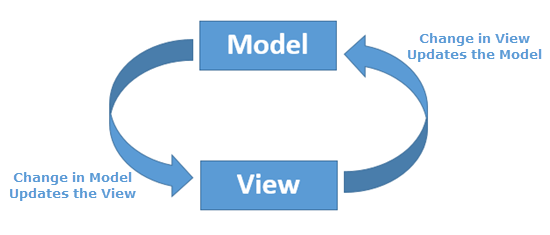
\includegraphics[width=\textwidth/2]{../immagini/twoWayBinding}
	\caption{Rappresentazione two way data binding.}
\end{figure}
\subsection{Gli eventi}
La libreria Ractive implementa il pattern architetturale  \textit{publish/subscribe}, che permette di rispondere o innescare particolari eventi, che attualmente vengono gestiti su due livelli.\\
Il primo è un interazione a basso livello con gli eventi del DOM che viene specificata tramite \textit{directives} del template che specificano anche  come l'evento deve essere gestito, tramite \textit{proxy event} o chiamate a metodi.\\
Il secondo è gestito dalle API \textit{publish/subscribe} e dal sistema di eventi all'interno di Ractive e tra i componenti.\\
I \textit{proxy events} collegano gli eventi del DOM con gli eventi di Ractive, mentre le chiamate a metodi direttamente sull'istanza ractive non utilizzano l'infrastruttura \textit{publish/subscribe}.
\subsection{Il virtual DOM}
Ractive utilizza un sistema differente dagli altri per tracciare le modifiche, ricorrendo al cosiddetto Virtual DOM, ossia a una rappresentazione virtuale della struttura del template immagazzinata in memoria e del tutto simile al DOM originale, del quale può essere vista come una astrazione.\\
Nel momento in cui si verifica un evento ed è necessario “reagire” ad esso modificando gli elementi della pagina, Ractive applica prima tali interventi al Virtual DOM.\\
Attraverso l’analisi delle differenze tra lo stato del Virtual DOM precedente al verificarsi dell’evento e quello nuovo ottenuto dall’applicazione delle modifiche, Ractive determina i cambiamenti effettivi da apportare al DOM vero e proprio.\\
Il calcolo delle differenze tra i due stati del DOM virtuale è estremamente veloce, e grazie a esso si limitano al minimo indispensabile gli interventi sul DOM reale, tendenzialmente più lento, garantendo quindi ottime performance.

\subsection{Plug-in di terze parti}\label{sec:packager}
I \textit{plug-in} permettono di aumentare le funzionalità offerte dalla libreria Ractive.\\
Agli sviluppatori è data la possibilità di creare i propri \textit{plug-in} o di scegliere quelli più adatti alle proprie esigenze da una lista presente sul sito di Ractive.js.\\
Durante lo sviluppo del progetto sono stati utilizzati i \textit{plug-in} \href{https://github.com/ractivejs/ractive-events-tap}{ractive-events-tap}, per gestire il click/tap sui dispositivi mobili , e \href{https://github.com/ractivejs/ractive-load}{ractive-load}, per il caricamento tramite protocollo \textit{http} dei template.   

\section{Sviluppo dei template}
La creazione dei template, per il progetto, non presentava nessuna restrizione né per la forma né per i contenuti, quindi la decisione di quali template sviluppare era a discrezione del programmatore.\\
L'unica richiesta, per questa fase del progetto, è stata quella di avere template sia HTML che SVG.\\
\subsection{Struttura ddei template}
I template HTML sono strutturati come una pagina web, cioè sono formati dal codice HTML per quanto riguarda i contenuti, il codice CSS per la loro rappresentazione grafica e JavaScript per definire il loro comportamento.\\
Il codice HTML rappresentante il template deve essere arricchito tramite la sintassi \textit{mustache} contenenti le variabili, le espressioni e le direttive necessarie al funzionamento del template.\\
Il comportamento del template viene sviluppato tramite gli strumenti offerti dalla libreria Ractive.
La libreria permette di creare un singolo file che contiene al suo interno l'intero template cioè HTML+mustache, CSS e Javascript.\\
Questo risulta molto vantaggioso in termini di quantità di file e organizzazione dei vari template.\\
Ogni template dovrà inoltre avere un file di tipo JSON contenente i dati da visualizzare ed eventuali immagini o librerie necessarie per il suo corretto funzionamento. 

\section{Rendere il template responsive}

\section{Inserimento plug-in jQuery nei template}

\section{Caricamento dei template nelle pagine HTML}

